\documentclass{article}
\usepackage{hyperref}
\usepackage{graphicx} % Required for inserting images
\usepackage{xcolor}

\title{MapReduce}
\author{Mark Doughten [md1875]}
\date{April 5, 2025}

\begin{document}

\maketitle
\section{Project Specification}

Project specification document (1--2 pages, due 04/02) outlining:

\subsection{Goal}
a clear, specific, measurable technical goal you can realistically achieve by the end of the semester;
existing prior work towards this goal;

\subsection{Description}
a description of how your project is novel, different, and/or builds on this prior work (there must be something new about what you do, however minor or incremental; just state it precisely);

\subsection{Outline}
a brief outline of the key technical idea or approach you intend to implement (it is suitable to draw system diagrams, list existing libraries and software you will use, etc.);

\subsection{Measurements}
a set of empirical, quantitative, and/or qualitative metrics you will evaluate your project on, and the methods you will use for your evaluation; and
any foreseen risks that may prevent you from achieving your stated goal.

\begin{figure}[ht]
    \centering
    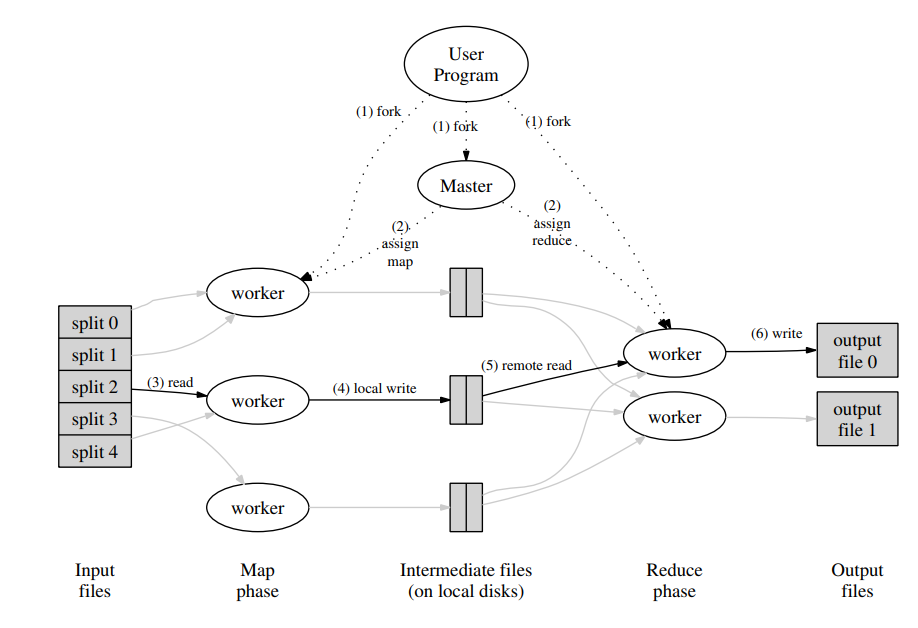
\includegraphics[width=1\linewidth]{./images/mapreduce.png}
    \caption{MapReduce \cite{mapreduce}}
    \label{fig:chroot}
\end{figure}

\begin{thebibliography}{}
\raggedright

\bibitem{mapreduce}
MapReduce.
\href{https://dl.acm.org/doi/10.1145/1327452.1327492}{https://dl.acm.org/doi/10.1145/1327452.1327492}

\end{thebibliography}
\end{document}
